\documentclass{article}
\usepackage{indentfirst}
\usepackage{graphicx}

\title{Shortcut to Knowledge: Answering Questions About Horse Racing with Data}
\author{Jack Karisch}
\date{June 2021}


\begin{document}

\maketitle

This paper documents my attempt to learn as much as possible about thoroughbred racing as I can by using data. My goal is to find a shortcut to the kind of knowledge veteran horseplayers accrue after years around the sport in a fraction of the time. The data is taken from Equibase results for all races run between January 1, 2020 and June 30, 2021. Each section will be a response to a basic question prompt that a curious spectator might ask about the sport. This paper will expand over time as I answer more of these questions.

\section*{How accurate are the odds?}

This is the most basic question a first-time bettor would ask. Like a stock price, the odds dictate the opinion of the market. In a system with perfect information, they would precisely predict the order of finish of every race. This obviously isn't the case, but how close do they get?

\begin{figure}
    \centering
    \textrm{Percentage of Runs Finishing in Position 1-6 For Six Favorites}\par \medskip
    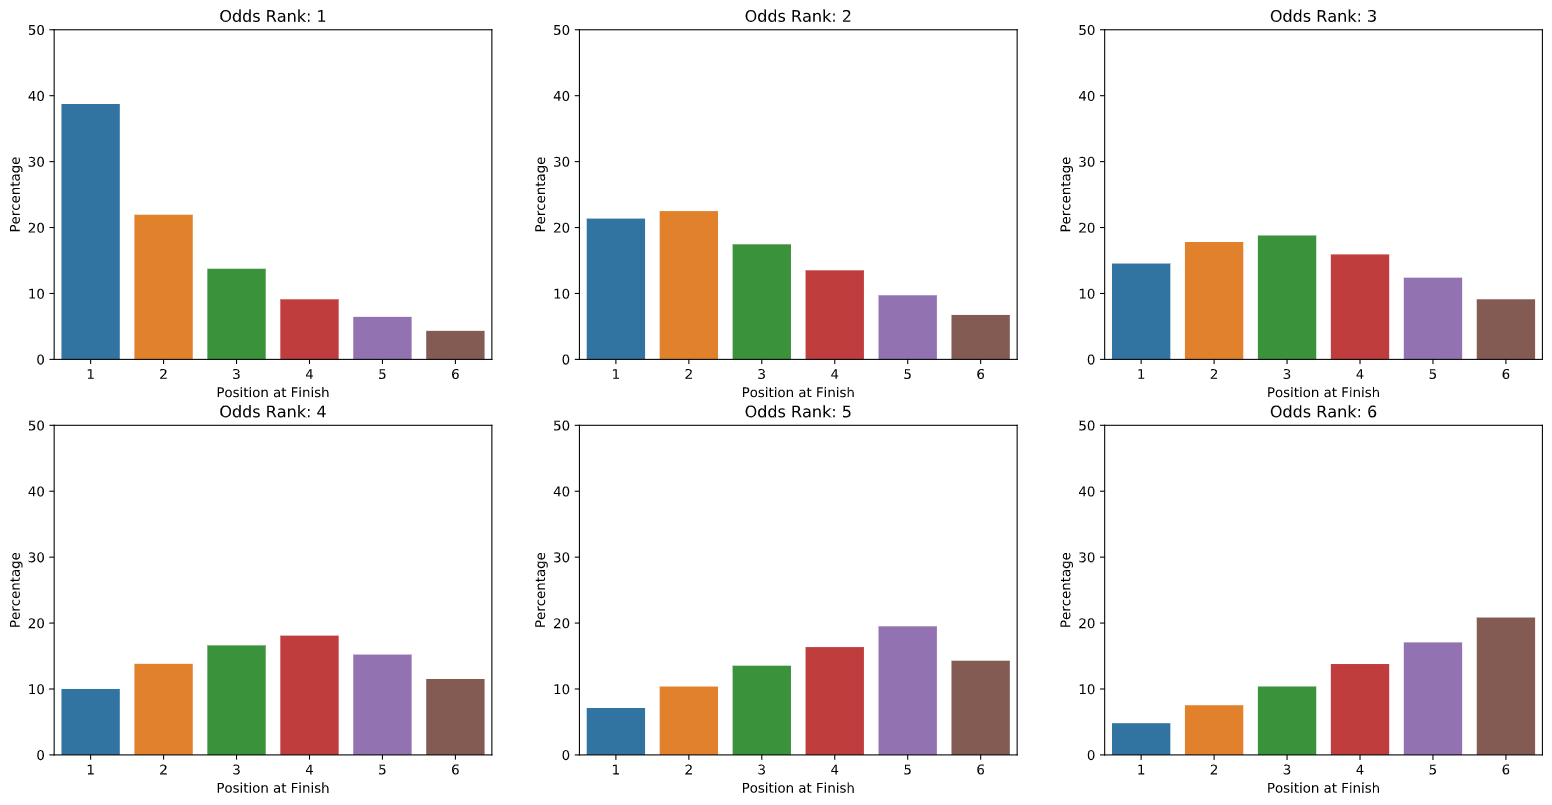
\includegraphics[width=12cm]{images/odds_rank_finish_chart.png}\medskip

    \caption{On average, the odds predict the order of finish, but there is a good deal of uncertainty}
    \label{figure:oddsRanksFinish}

\end{figure}

Figure \ref{figure:oddsRanksFinish} provides a very basic answer to this question. The favorite won in 39\% of races, placed in 61\% and showed in 74\%. The second favorite placed in 44\% of races and showed in 63\%. The third favorite showed 51\% of the time. In general, the odds do predict the order of finish (at least through the first 6 positions), but with a lot of uncertainty. The odds predict the winner with much more success than they predict any other finisher, which makes sense because that's exactly what bettors are trying to do; it makes no difference to a gambler if his horse finishes second or dead last if he places a win bet.

\begin{figure}
    \centering
    \textrm{Distribution of Raw Odds and Lengths Back Variables}\par \medskip
    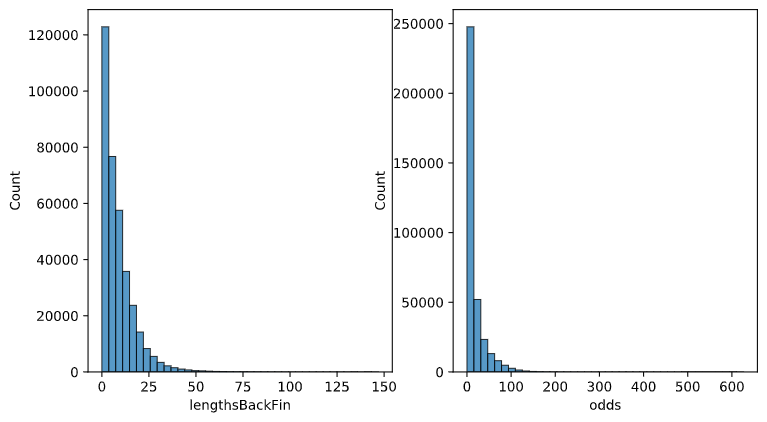
\includegraphics[width=12cm]{images/lengths_odds_no_trans_chart.png}

    \caption{The untransformed distributions show heavy skew} 
    \label{figure:oddsLengthsNoTrans}   
\end{figure}

In order to check whether the odds can predict the relative performance of the horses, we turn to linear regression. The goal is to find the effect of increasing odds on the number of lengths back from the leader a horse finishes. Figure \ref{figure:oddsLengthsNoTrans} shows the distribution of the variables encoding odds and number of lengths behind leader at the finish of the race. Both of these distributions show aggressive right skew.  so they are poor candidates for a linear regression fit. The lengths back variable shows this pattern because horse racing is designed in such a way that all the horses finish as closely as possible to one another. The odds variable shows the pattern because the standard deviation increases as the odds increase. 

\end{document}